\section{Identifying mutations in ESBL \textit{E. coli} accumulated by evolving resistance against cefepim}
We established a pipeline which allowed us to identify mutations which accumulated by evolutionary pathways while an ESBL \textit{E. coli} strain changed their phenotype from susceptible to resistant to cefepime. Thise pipeline was based on sequencing data coming from multiple samples which were taken along the evolution of resistance. Samples token along this pathway are also referred as sample series. The steps of the pipeline are shown in Figure \ref{figure:pipeline}.

\subsection{Creating a reference genome with annotation} 
The first step was to de novo assemble the genome of the sample with the lowest cefepime MIC of a sample series which we called reference genome. We did that by hybrid assembling long-read sequencing data produced with Oxford Nanopore Technologies (ONT) and short-read Illumina sequencing with Unicycler \cite{wick_unicycler:_2017}. Nnaopore sequencing was done by ourselves, Illumina sequencing by our collaborators of the University Hospital of Basel.  

\subsubsection{Oxford Nanopore Technology sequencing}
For ONT sequencing the library was prepared with a ligation sequencing kit (LSK-108) followed with the native barcoding expansion kit. This allowed barcoding of multiple samples and loading all of them on a single flow cell (FLO-MIN106D). As a sequencing device we used the MinION from ONT. \\
As a fist step each DNA isolate was diluted to a concentration of 1 \textmu g/\textmu l in 50 \textmu L nuclease free water (NFW). For end-repairing the DNA 7 \textmu L NEBnext Ultra II Endrepair/dA-tailing enzyme mix were added to each
sample and incubated at 20\degree C for 5 min and at 65\degree C also for 5 min. After this step every sample was cleaned up by adding 60 \textmu of AMPure XP beads. The beads were incubated with the samples for 5 miuntes ona a rotor and then removed on a magnetic rack. Every sample was washed with 200 \textmu L 70\% ethanol which was repeated once. The ethanol was removed and every sample was suspended in 25 \textmu L NFW. 2.5 \textmu L of each barcode plus 25 \textmu L of Blunt/TA ligase was added to each sample and incubated for 10 minutes. All the samples were pooled and 500 \textmu of AMPure XP beads were added. After incubating the pooled sample for 5 minutes on the rotor the sample was washed again twice with 70 \% ethanol. All the DNA was eluted in 51 \textmu L NFW. The final sample was diluted to a concentration of 35 ng/\textmu L. Then for adapter ligation 20 \textmu L BAM, 30 \textmu L Ultra II ligation master mix and 1 \textmu L enhancer were added. After 10 minutes of incubation, 40 \textmu L AMpure XP beads were added and incubated on the rotor for 5 minutes. The supernatant was removed on the magnetic rack and the DNA was washed twice with ABB. The DNA was eluted and incubated for 10 minutes in 15 \textmu L ELB. Finally the library was prepared by mixing 15 \textmu L of eluted DNA in ELB with 25.5 \textmu L LLB and 35 \textmu L RBF. The resulting library was loaded on the flow cell, which was primed before with a mixture of 480 \textmu L RBF  and 520 \textmu L of NFW. The sequencing run was started and simultaneously base-called with Albacore.

\subsubsection{Illumina sequencing}
The DNA from the samples was isolated using the EZ1 DNA tissue kit on an EZ1 Advanced XL robotic system (Qiagen). The library for the sequencing was prepared using the Nextera XT library preparatino kit (Illumina) and the resulting library was sequenced on a MiSeq Illumina platform \cite{nanopore}. The reads produced with Illumina were trimmed with Trim Galore \cite{noauthor_babraham_nodate}.

\subsubsection{Annotating the reference genome}
Every reference genome was annotated with prokka (v.1.12) \cite{seemann_prokka:_2014}. Additionally promotor regions were identifed using the promoter prediction tool PePPER \cite{pepper}. PePPER is a tool which takes whole-genomes as an input and predicts promotor sequences. Those sequences were mapped against the reference genome using graphmap \cite{sovic_fast_2016}. Furthermore a promotor data base hosted on EcoCyc was used which contains around 3800 experimentally validated promotors for \textit{E. coli}\cite{noauthor_smarttable_nodate}. The sequences from this database were downloaded and mapped against the reference genome with graphmap aswell \cite{sovic_fast_2016}. 
\label{section:annotatiion_ref}

\subsection{Mapping Illumina sequencing data of the sample series to the reference genome}
As a second step the short-read Illumina sequencing data of every sample from the sample series was mapped against the reference genome of the sample series. Mapping to the reference genome was done with BEW mem \cite{li_fast_2009}. This step established the base to identify mutations. This is because we could check the most abundant base of every Illumina read mapped to a certain positions. If the most abundant base in a resistant sample differs a mutation was present. To make this information more accessible we calculated pile-ups as a third step of our analysis. 

\subsection{Creating pile ups}
Pile-ups are count matrices which store which base is present how many times at a certain position considering every Illumina read mapped to this position. In order to produce those pile-ups we used a script called \href{https://github.com/nahanoo/ESBL\_project/pileup.py}{pileup.py} Because the same reference genome was used for all the samples from one patient all the pile-ups from one patient could be stored in a matrix stack. This allowed us to easily calculate base frequencies, coverage or to identify the most abundant base at a certain position of a sample. This data construction also allowed us to easily compare the most abundant base at a position in all the samples.

\subsection{Identification of mutations} 
We identified mutations by comparing the most abundant base at every position for every sample of the matrix-stack with a script called \href{https://github.com/nahanoo/ESBL\_project/pileup.py}{analysis\_modular.py}the pile-ups of all samples from one patient. If the most abundant base varied a SNP was identified. This way were able to find SNPs, deletions of any length and insertions.
For the rest of the pipeline only mutations were included where the coverage was at least 30 and the base frequency at least 0.8.

\subsubsection{Identification of genes and promotors affected by SNPs}
As a last step of the pipeline it was checked if annotation was available for every found mutation. As described in section \ref{section:annotatiion_ref} genes and promoters were identified for every reference genome. \\
For checking if a SNP affected a gene, we analyzed the genbank file with biopython \cite{cock_biopython:_2009}. We checked if a mutation was located between a start and an end position of a gene. For checking if a SNP affected a promotor region we analyzed the bam-files which were created with the promoter sequences coming from PePPER and EcoCyc (see \ref{section:annotatiion_ref}). We checked if a SNP was loacted between a start or end positon of a mapped promotor sequence. 

\subsection{Overlap based whole-genome assembling}
For one sample series we tried another assembler called canu \cite{koren_canu:_2017}. Canu is an assembler which assembles the whole-genome based on overlaps of the long-reads. Illumina-reads can be used to polish errors in the assembly from canu. Polishing is possible with the software called pilon \cite{noauthor_pilon:_nodate}.


\section{ESBL \textit{E. coli} sampling at the University Hospital of Basel}
Our collaborators from the clinical microbiology of the University hospital of Basel collected 65 \textit{E. coli} samples of 34 patients. Those collected samples were all screened positive for ESBL genes. This resulted in ESBL \textit{E. coli} sample series with one to four samples per patient. The sampling period was between 2011 and 2015. Sample collection for one patient typically happened within several months.
\subsubsection{Screening for ESBL genes}
Coming after meeting with Adrian
\subsection{Selection of samples suitable for our analysis}
Our collaborators determined the MICs of every sample for the third-generation cephalosporin ceftazidim and the fourth-generation cephalosporin cefepim. Some sample series showed a significant change of the MICs. Sometimes resistance was gained, but in certain cases resistance was also lost. We were interested in identifying mutations in sample series where susceptibility significantly changed and all the samples from a series were the same ESBL \textit{E. coli} strain.
\subsubsection{Determination of the minimal inhibitory concentration}
Coming after meeting with Adrian.

\subsection{Pylogenetic analysis}
We checked if a sample series were the same ESBL \textit{E. coli} strain by running a phylogenetic analysis with Illumina sequencing data. For phylogenic analysis we used a tool called PanX \cite{ding_panx:_2018}. Illumina data for every sample was provided by our collaborator.
\subsubsection{Illumina sequencing}
The DNA from the samples was isolated using the EZ1 DNA tissue kit on an EZ1 Advanced XL robotic system (Qiagen). The library for the sequencing was prepared using the Nextera XT library preparatino kit (Illumina) and the resulting library was sequenced on a MiSeq Illumina platform \cite{nanopore}. The reads produced with Illumina were trimmed with Trim Galore \cite{noauthor_babraham_nodate}.
\subsubsection{PanX}
PanX is a tool which clusters samples based on their genes into orthologous clusters. From those clusters, panX identifies the core genome which are genes shared by all samples in the cluster. Based on those core genomes a strain-level phylogeny can be build, making use of single nucleotide polymorph positions (SNPs) within the core genomes. \\ 
PanX used annotated whole-genomes as input files that is why every sample was short-read assembled and annotated. For short-read assembling we used spades (v3.12.0) \cite{nurk_assembling_2013}, for annotating the resulting assemblies we used prokka (v.1.12) \cite{seemann_prokka:_2014}. Prokka first searches a core set of well chacracterized protein using BLAST+ and then compares reading frames to a database derived from UniProtKB \cite{seemann_:zap:_2019}. The results from prokka were stored in a genbank file for every isolate. Based on those genbank files the PanX analysis was performed. \\



\newpage



\section{Assembling and handling procedure of the morbidostat}
The following system is an adapted version of Topraks built differing mainly in its pump system, controlling unit and software. Hardware which was not commercially available was built by the in-house mechanic and electronic workshop.

\subsection{Hardware and setup}

\begin{figure}[H]
	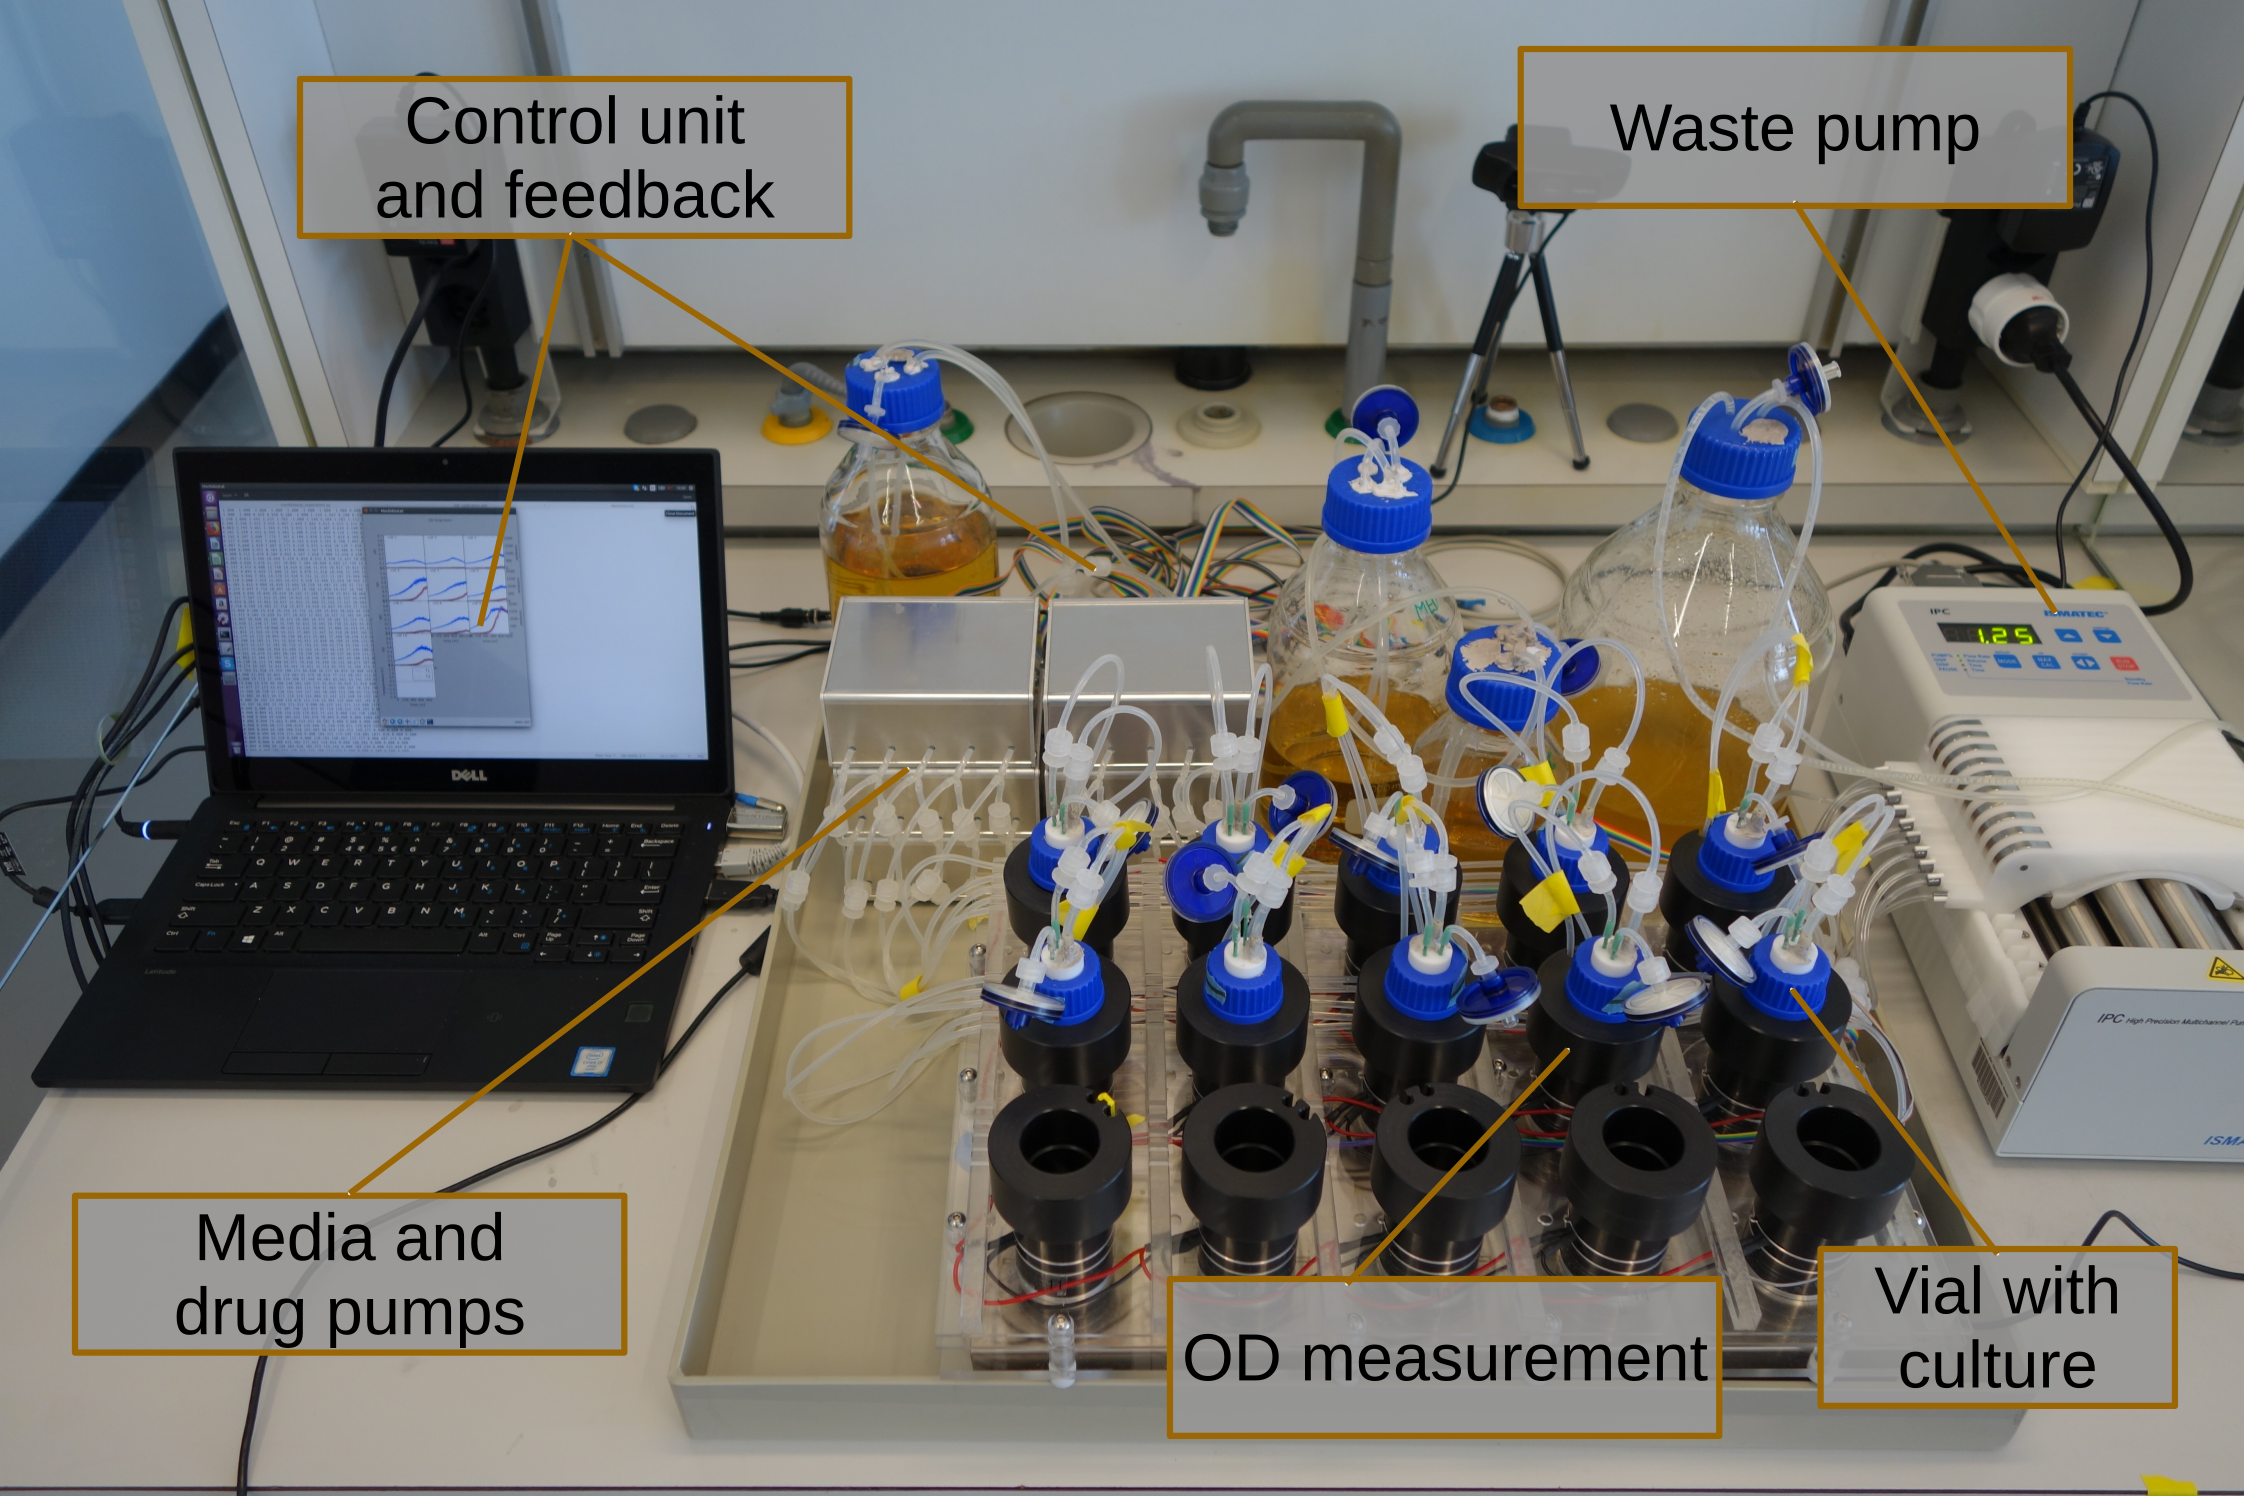
\includegraphics[width=0.6\textwidth]{setup_annotated_inksacpe.png}
	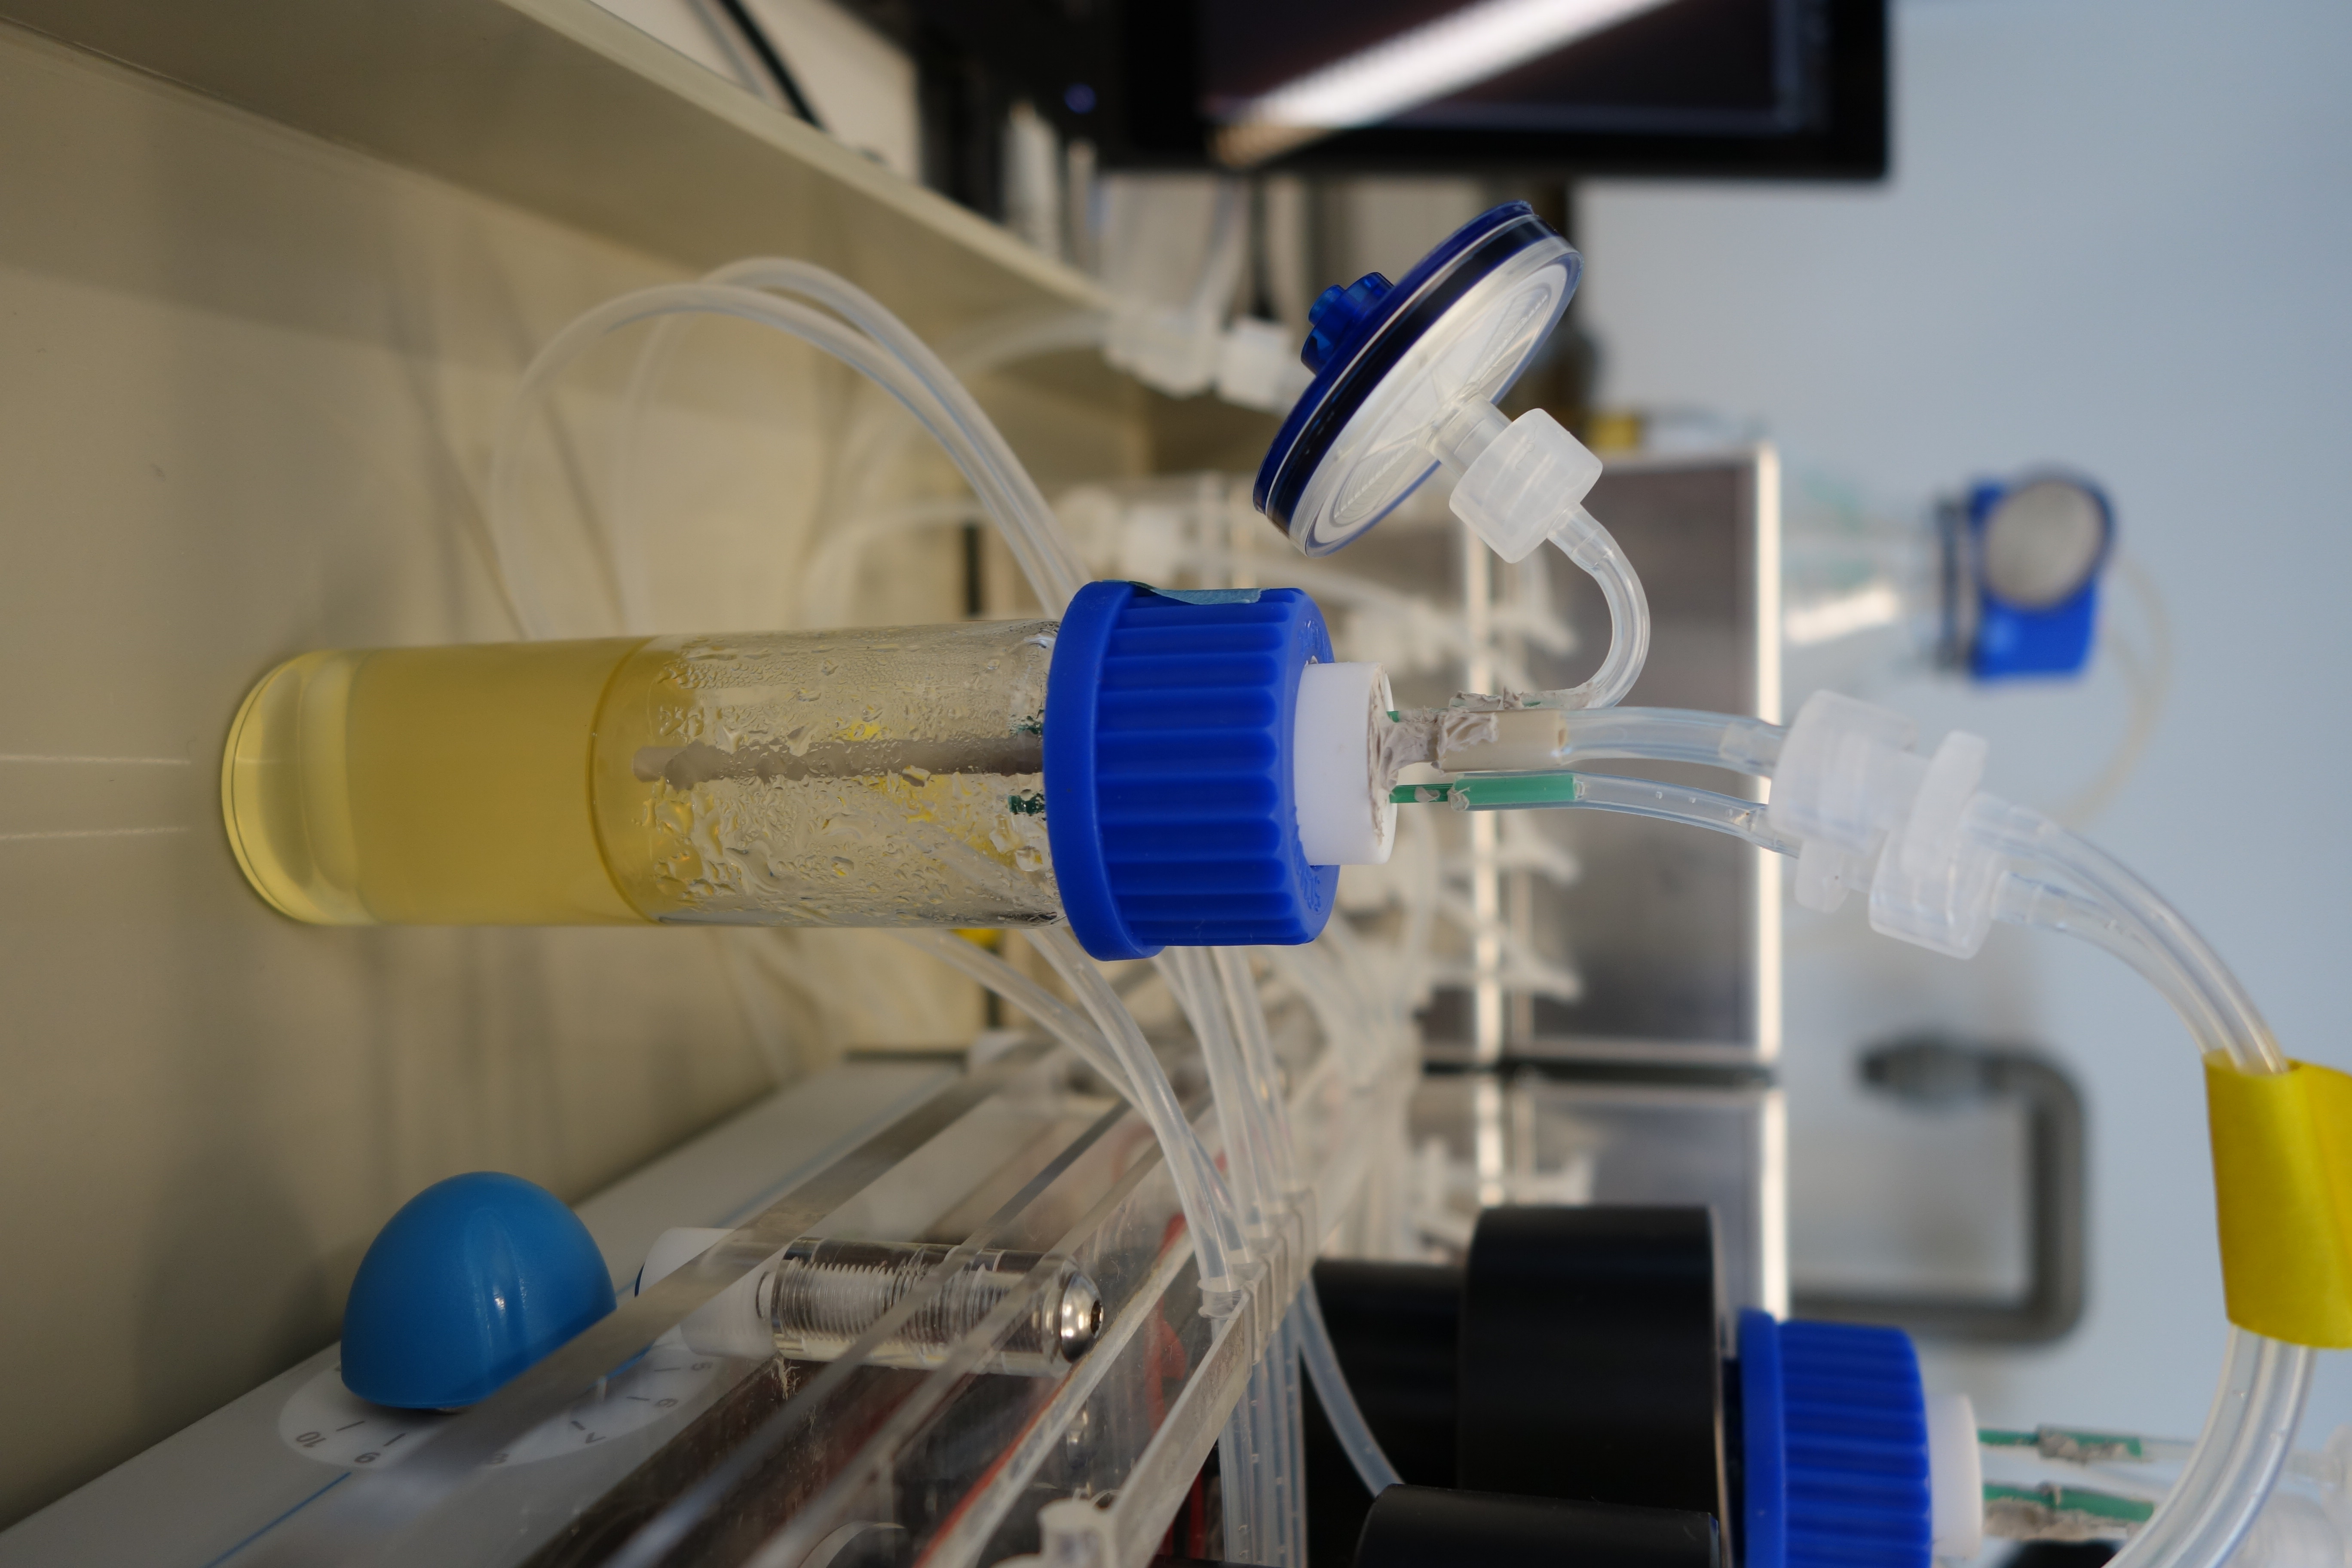
\includegraphics[width=0.4\textwidth,angle=90]{vial.JPG}
	\caption{Left: Overview of the morbidostat setup. The microcontroller is located behind the drug and media pumps. Right: One vial with all the inlets.}
	\label{figure:morbidostat_setup}
\end{figure}  
Figure \ref{figure:morbidostat_setup} shows the morbidostat setup.
As a base for our built we used a magnetic stirrer with 15 slots. On that stirrer we placed three layers of acrylic glass which acted as our vial holders. Between the acrylic glass layers the OD measuring units  were installed.  To block out as much light as possible, the vials were surrounded with black plastic rings as visible in Figure \ref{figure:morbidostat_setup}.
The vials placed in the vial holders had three inlets. One inlet was used to inject media or antibiotics, through another one exceeding volume was removed and the last one was used to mount an air filter for pressure equilibration.  Even though only one tube per vial was used for injecting fluids each vial was connected to three injecting pumps. Every pump was connected to a bottle with media, a low-concentrated and a high-concentrated antibiotic solution. The tubing from the three pumps per vial was connected to one and led to the vial. Injection of the desired concentration was possible by turning on pumps for certain times. In order to control the pumps and to measure the ODs we used a mircocontroller. We connected the microcontroller serially to a PC. The programs on the PC were responsible for initializing morbidostat hardware commands and to store injected antibiotic concentrations as well as measured ODs. This allowed us to see approximately how much resistance was already gained at any time-point of the experiment. \\
For assembling and testing the hardware we built the morbidostat in the open as shown in Figure \ref{figure:morbidostat_setup}. For the actual experiments we placed the morbidostat insite an hypoxi-station in a bio safety lab 2. This allowed us to culture the bacteria at 37 \degree C but also to increase the safety. 


\subsubsection{Measuring of optical densities}
For measuring the OD a combination of a light emitting diode (LED) and a phototransistor was chosen. We chose OPB608A as a LED with a peak wavelength of 890 nm and PT 333-3C as a phototransistor, both from from TT electronics. We made use of the fact that cells cause scattering of a ray of light. For each vial we placed a LED and aphototransistor at the glass wall of the vials orientated in a 135 \degree \space angle towards each other. The LED was constantly on shining light through the cultures. When an OD measurement was initialized by the microcontroller the scattering of the light beam was measured with the phototransistor. LEDs and phototransistors were both connected to independent 5 V circuits. Additionally the OD measuring units were grouped in three groups with five vials corresponding to one row of vials. This means that every row of vials had an independent LED and phototransitor circuit. The circuits of one row of the morbidostat are illustrated in Figure \ref{figure:OD_cirguit}, where the LED circuit is shown orange and the photoransistor cicruict in blue. We connected the five LEDs in parallel and placed a x \textOmega resistor after the LEDs. The circuit of the phototransistor was also build in parallel. Each phototransistor had a potentiometer connected in serial, over this potentiometer the voltage was measured. 
Measuring the scattering worked as follows. Light reaching the phototransistor caused an opening in the semiconductor from the phototransistor which led to an amplification of the current by the transistor. This current reached the potentiometer over which we measured the voltage. The opening of the semiconductor was proportional to the light which reached it. More cells in the suspension caused more scattering, meaning a bigger opening in the semiconductor. A bigger opening led to more current. If more current reached the resistor, the measured voltage was smaller. This means that the measured voltage was proportional to how many cells were in the suspension. By calibration we could translate the voltage to an OD. In order to do so we measured different OD standards with a known OD and stored the corresponding voltages. Measuring multiple OD standards allowed us to calculate a linear equation. This equation was used to convert the voltages to ODs. 
We chose a potentiometer in order that we can change the sensitivity by changing the resistance over which we measured the voltages. It turned out that the system was not as sensitive as thought in advance, so all the potentiometers were opened as much as possible meaning that the highest possible resistance was chosen.   

\begin{figure}
	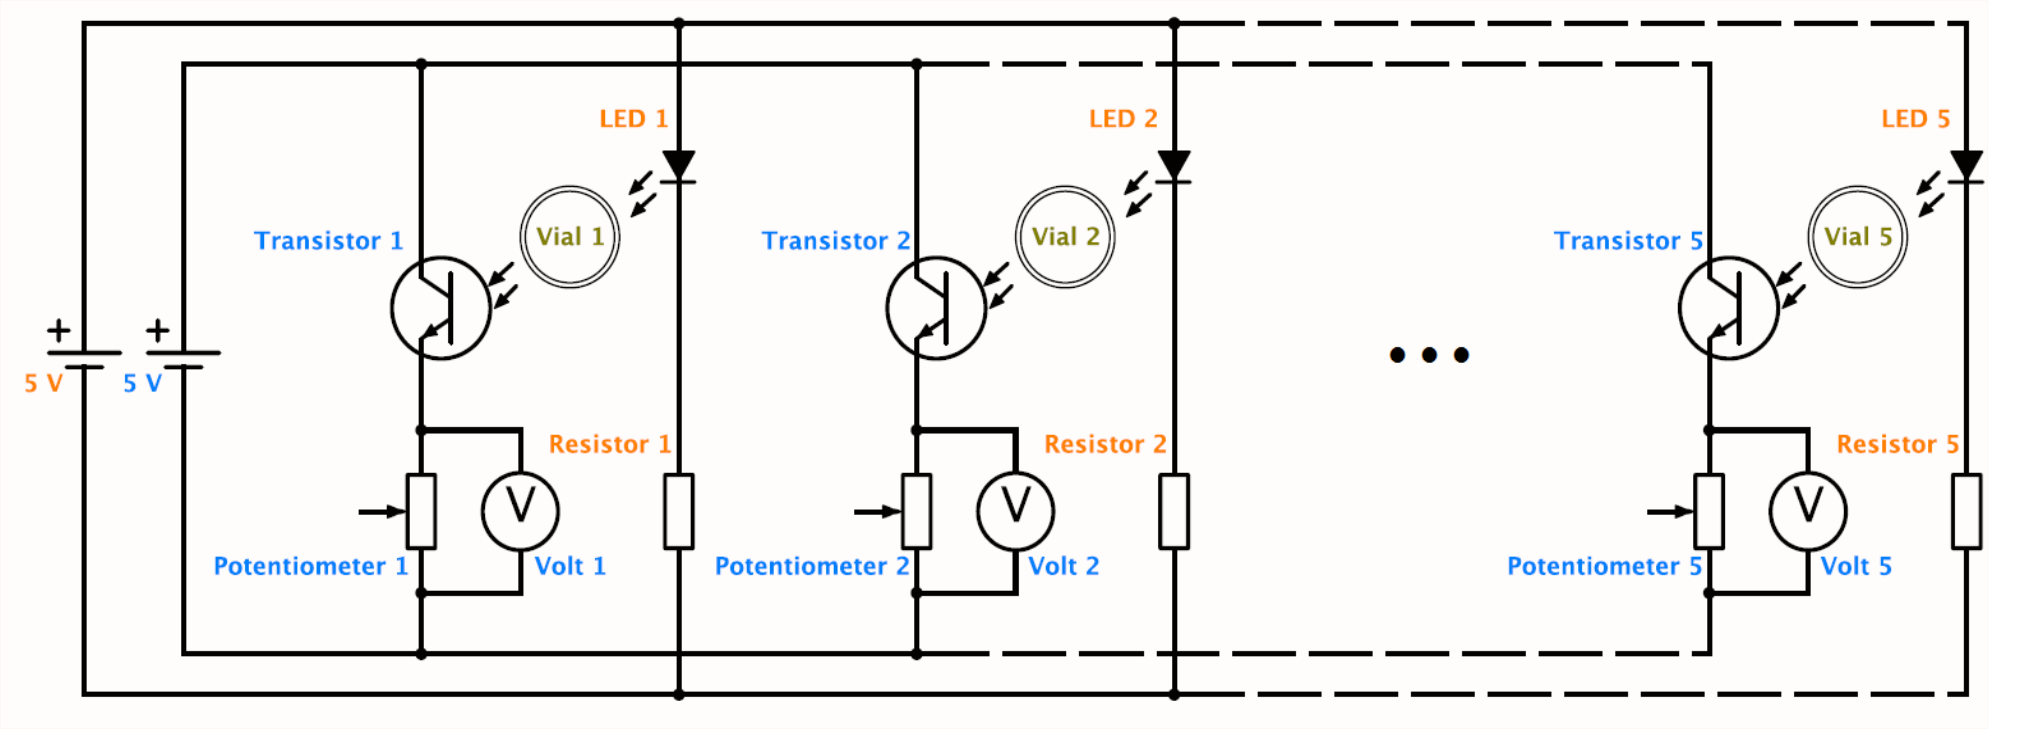
\includegraphics[scale=0.15]{OD_setup.png}
	\caption{Circuit diagram of parallel-connected LED (orange) and phototransistors (blue). This circuit is done independently three times for five vials each. The detector and the LED are orientated in a 135 \degree  angle since this is the best angle for detecting light scattering.}
	\label{figure:OD_cirguit}
\end{figure}

\subsubsection{Pumps and tubing} 
\begin{figure}
	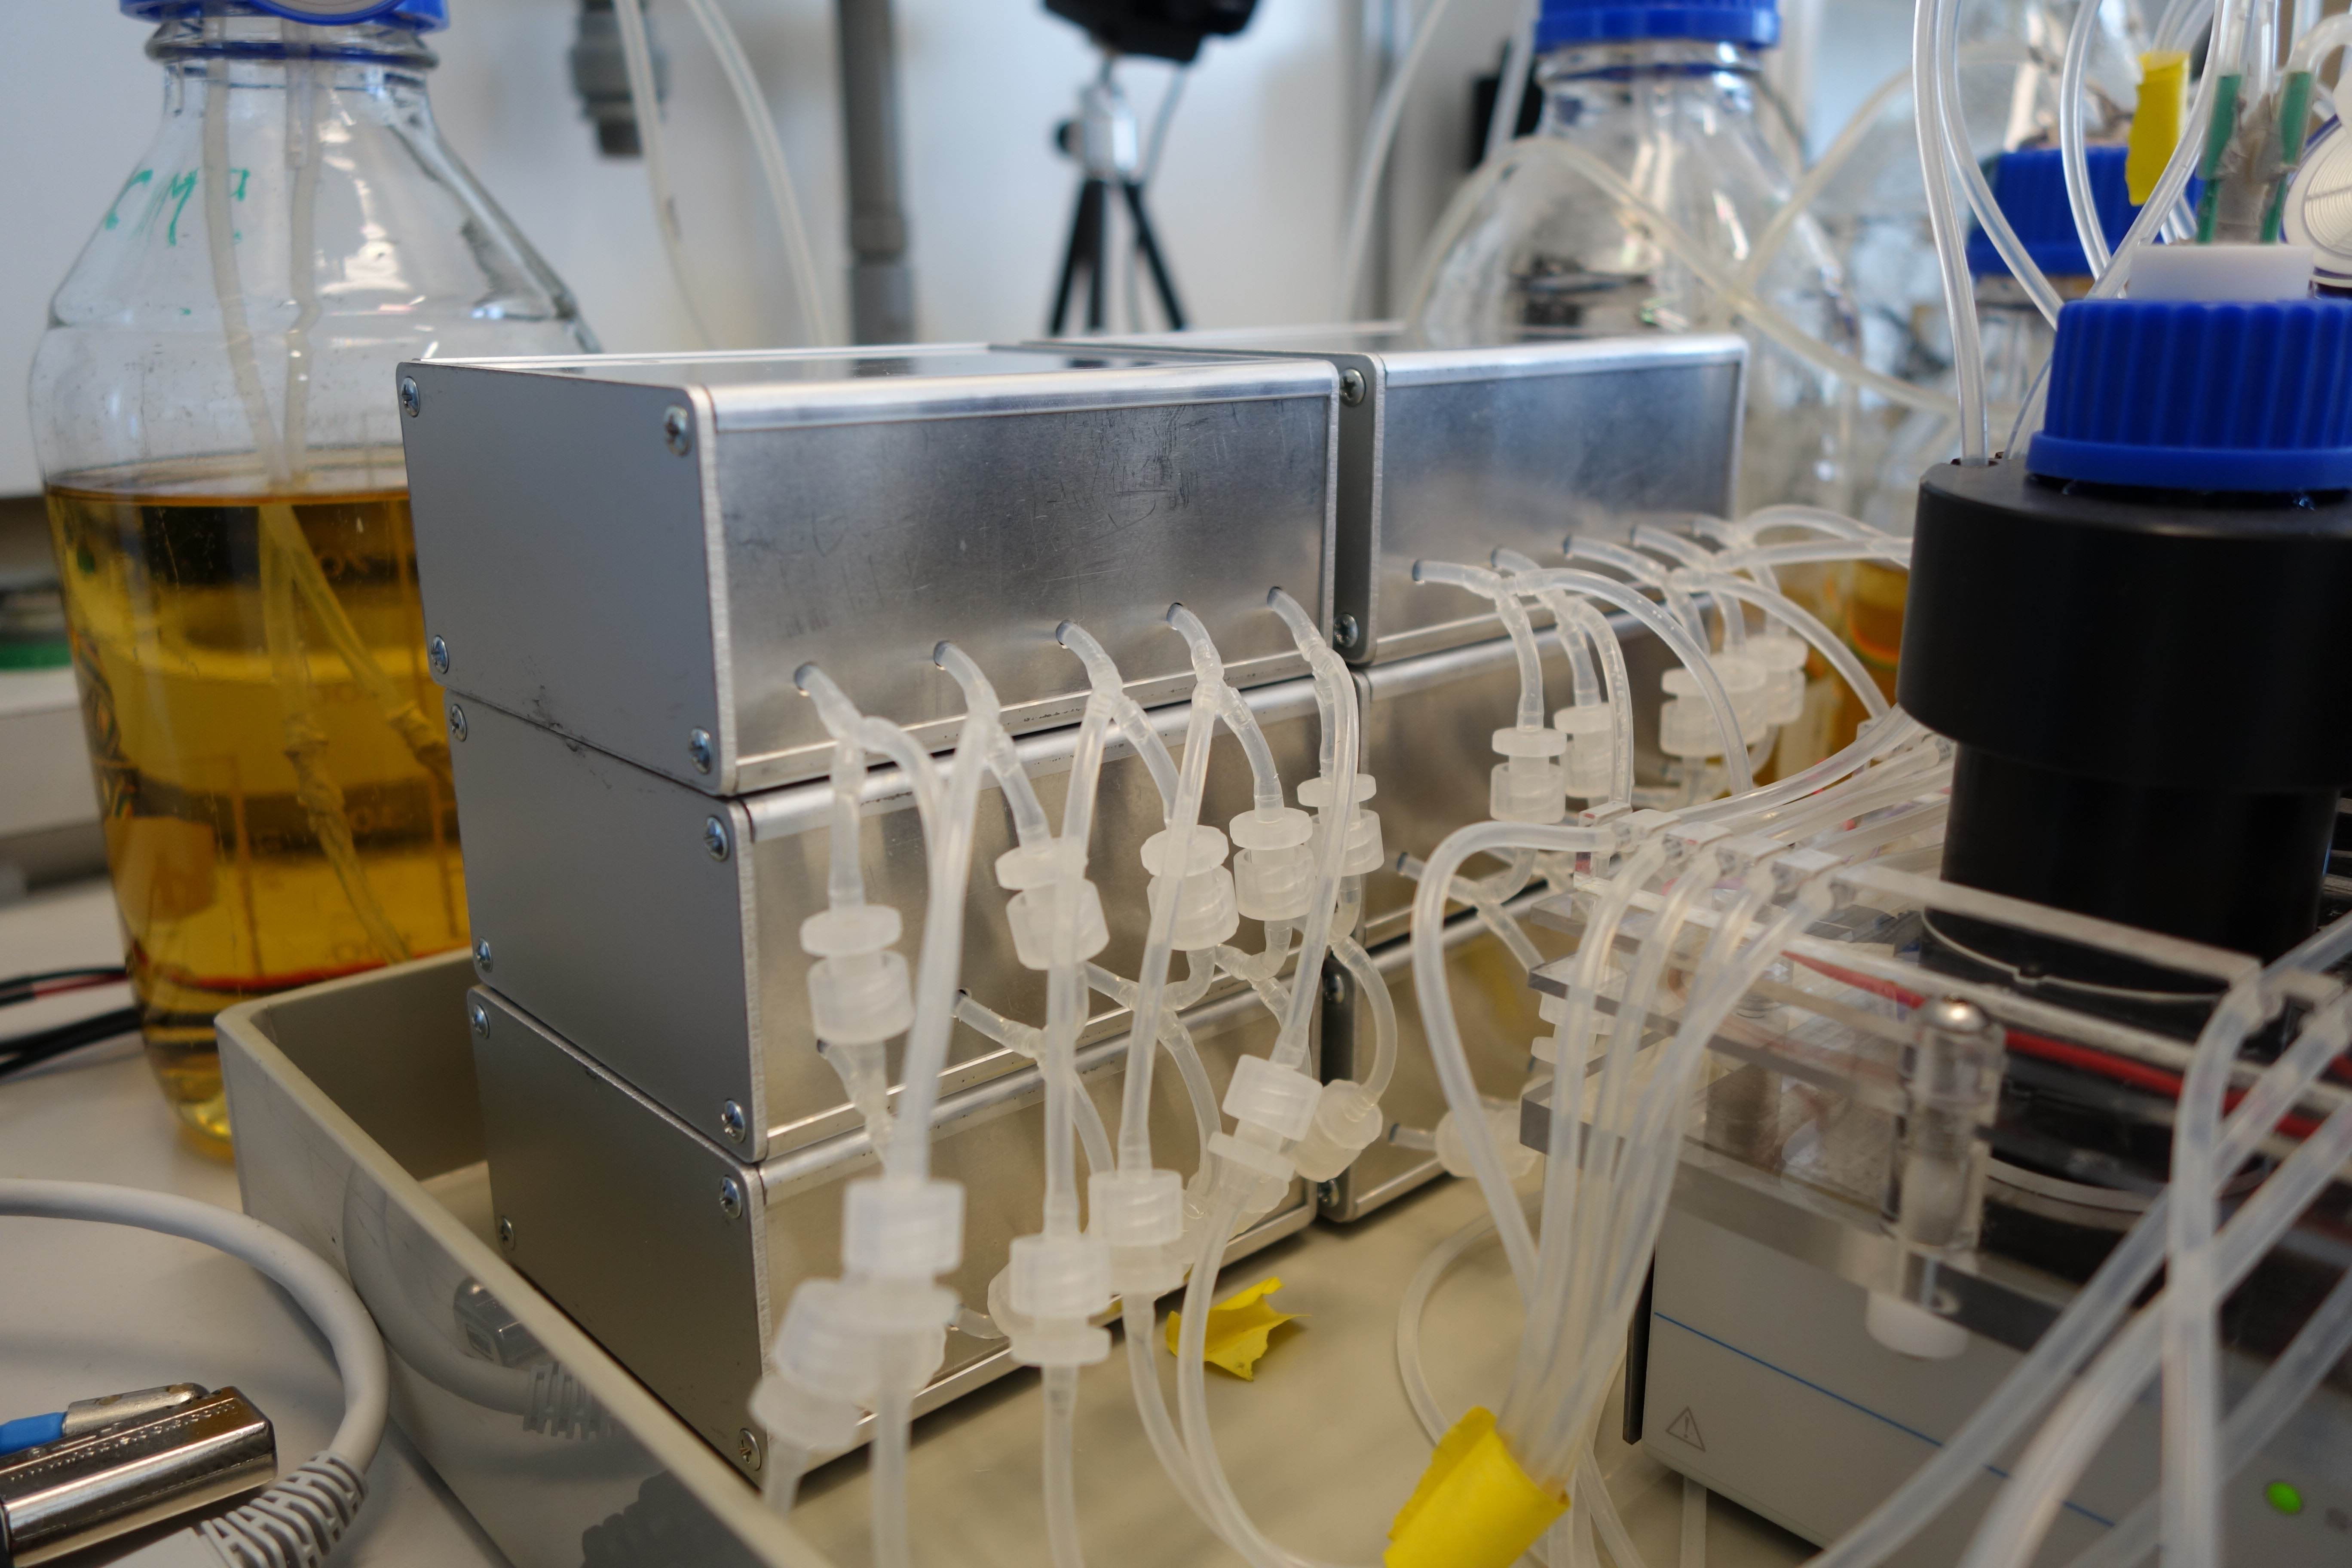
\includegraphics[scale=0.226]{pump_blocks.JPG}
	\caption{Figure left: Vial setup. Figure right: One row of five pumps represents one row of five vials. Since every vial is connected to three pumps, three rows of pumps are stacked on top of each other and connected column by column. This means that one column of three pumps is responsible for injection fluid into one vial. Every outlet from a pump from one column is connected, in order that there is just one tube going to one vial. }
	\label{figure:tubing_setup}
\end{figure}
Three connected injecting pumps per vial led to 45 injecting pumps in total. Mp6 pumps from microComponents were chosen because they have a compact built, having the size of half an USB stick. This is an improvement because the pumps used by Toprak et al \cite{toprak_building_2013} and Doesselmann \cite{doselmann_rapid_2017} were peristaltic pumps which were cubic with a size of approximately 4x4x4 cm. 

The functional principle is based on a piezoelectric diaphragm in combination with passive check valves which is shown in figure \ref{figure:piezo}. By applying voltage a piezo ceramic mounted on a membrane is deformed resulting in a down stroke. When the voltage decreases again the piezo deform again causing an upstroke of the membrane \cite{piezo_pumps}. Because the pump process depends on excitement and relaxation caused by the power, the flow rate generated by the pumps is dependent from the frequency. This also implements that the flow rate is very constant given that the power frequency is also constant. That being the case, the mixing of drug concentration was done by turning on the pumps for a calculated time.

In order to excite and relax the piezo ceramic 230 Volts and a very steady power frequency were needed for this process, making it necessary to control every single pump with a specific mp6-OEM controller. This controller took an input power of 5 V and used about 30 mA of current. The Arduino was not capable of supplying this amount of current for every pump, therefor a separate power adapter was installed to supply the pumps. 

The pumps could be controlled by connecting one pin of the controller from the pump to a digital pin of the Arduino. 
If the pin from the controller was put to ground, the pumps were turned on, if the pin was connected to 5 V the pumps were off. Turning on/off the controller only worked well, when the change of power was very sudden. 
By adding a pull-down resistor between the digital pins and the ground from the Arduino we could avoid that there was always a very small current flowing through the digital pins. Furthermore it was decided to work with a serial connected inverter, implementing that when the digital pin was set to low, the inverter caused a power of 5 V which meant that the pumps were off. On the other hand when the digital pin was set to high, the inverter produced a power of 0 V which turned the pumps on.  
As a waste pump a 16-channel peristalitc pump was used which was directly controlled with a digital pin from the Arduino. 
\label{section:pumps}
\begin{figure}
	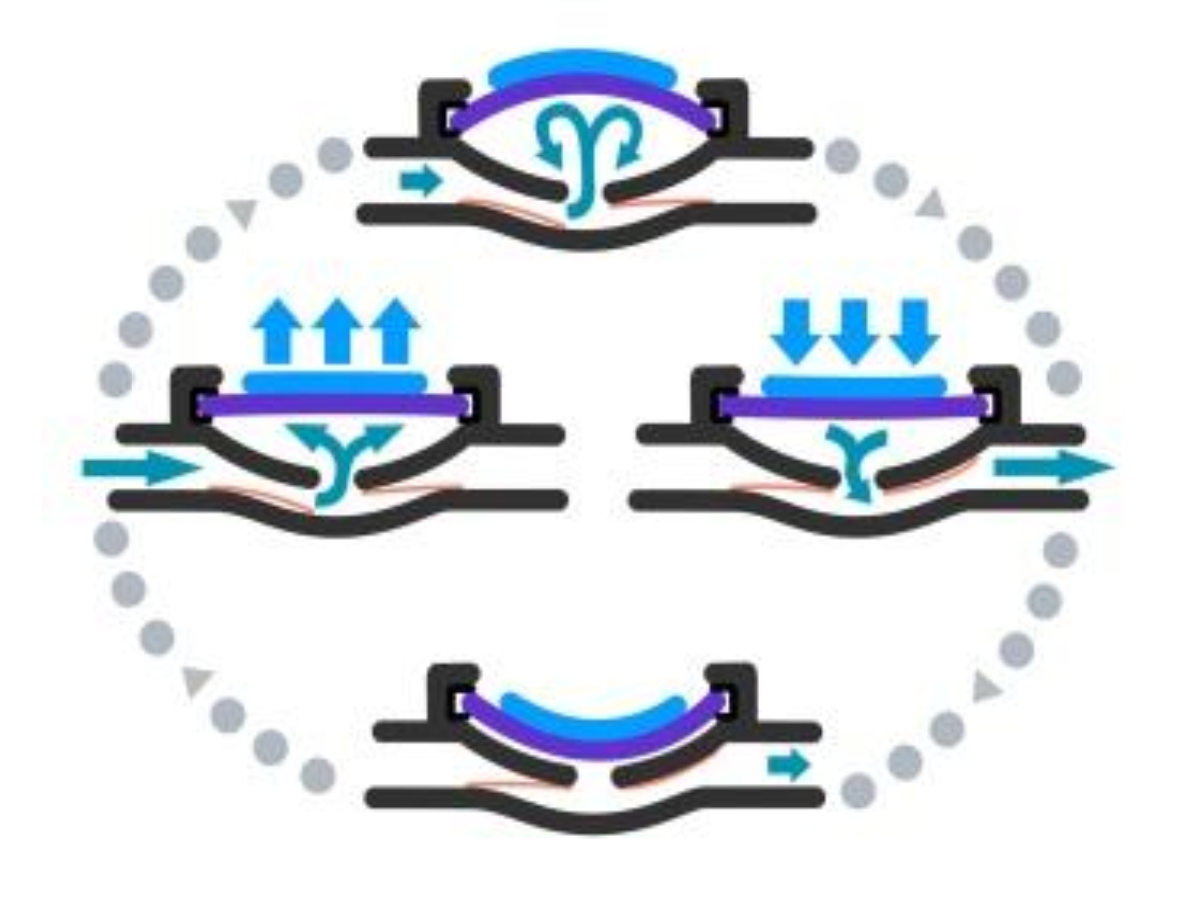
\includegraphics[scale=0.1]{piezo.png}
	%\includegraphics[]{circuit board}
	\caption{Principle of the mp6 pump but two of those piezoelectronics are connected in serial for this pump model \cite{piezo_pumps}}
	\label{figure:piezo}
\end{figure}

\subsection{Morbidostat modes and control}
One mode was growth\_rates which we used in order to record growth rates, in this mode nothing was injected into the vials. Another mode which we called fixed\_OD kept the cultures at a desired OD by diluting the culutres with the right amount of media. The last mode was called continuous mode and is the mode that we used to force bacteria to gain resistance. To each vial a different mode could be assigned. 
We implemented three different modes for culturing bacteria with the morbidostat. CONTINUOUS\_MORBIDOSTAT (C) allows to automatically culture bacteria while constantly inhibiting growth with antibiotics. GRWOTH\_RATE\_EXPERIMENT (G) simply recorded and stored the growth rates of growing bacteria without adding any fluid. FIXED\_OD\_EXPERIMENT (OD) lept diluting the cultures only with media in a way that the cultures stayed at a fixed OD.
Within the same experiments different modes could be used for different vials. A detailed manual for how to start morbidostat experiments from the command line is available in the Section \ref{section:manual}. The following paragraphs describe the scripts and command chains which controlled the hardware. \\

\subsubsection{Hardware control and data management}
The control of the morbidostat was divided into two python scripts running on the laptop and one .ino script running on the microcontroller. Every script is available on \href{https://github.com/nahanoo/ESBL\_project/}{GitHub}. On the laptop all the scripts are located at \newline /home/morbidostat/python\_morbidostat/python\_src/.
Communication of the latop on the microcontroller was possbile via an USB cable enabling serial communication.
The two python scripts were arduino\_interface.py and morbidostat\_experiment.py. The arduino\_interface.py was responsible for transmitting commands to the microcontroller via the the serial connection but also for receiving data from the microcontroller. The morbidostat\_experiment.py script on the other hand was responsible for saving data, initializing cycles and calling different functions depending which mode was chosen.The arduino\_morbidostat.ino code interpreted and executed the commands received from the laptop. Those commands were measuring voltages of analog pins, needed for the OD measuring, or truning on/off digital pins which turned the pumps on/off (see section \ref{section:pumps}).


\subsubsection{Command flow of the continuous mode} 
As for every mode the continuous mode consisted of several steps which were grouped in one cycle. Those cycles were constantly executed. As shown in Figure \ref{figure:flowchart} the cycle itself was initiallized by morbidostat\_experiment.py and the ODs were measured and saved for every vial over the defined cycle time (typically 10 minutes). \\
Measuring of the OD as initialized by morbidostat\_experiment.py led to a function call in arduino\_interface.py which transmitted a command to the arduino. This command got interpreted and lead to measuring the voltages of the analog pins which were connected to an OD measuring unit as shwon in top right of the Figure \ref{figure:flowchart}. The resulting voltages got transmitted to the arduino\_interface.py via the serial communication. This script translated the voltages to ODs according to a linear equation defined earlier by calibration. Morbidostat\_experiment.py was responsible for saving the ODs and averaging those values at the end of the cycle. As a next step a function in morbidostat\_experiment.py calculated how much drug should get added to which vial, based on the recorded ODs. The output of the function were runtimes of certain pumps. Those runtimes were transmitted again to the arduino via the arduino\_interace.py script and interpreted by the arduino. As shown in the last illustration of Figure \ref{figure:flowchart} the arduino switched the according digital pins to high for the time communicated from the laptop.
 
\begin{figure}
	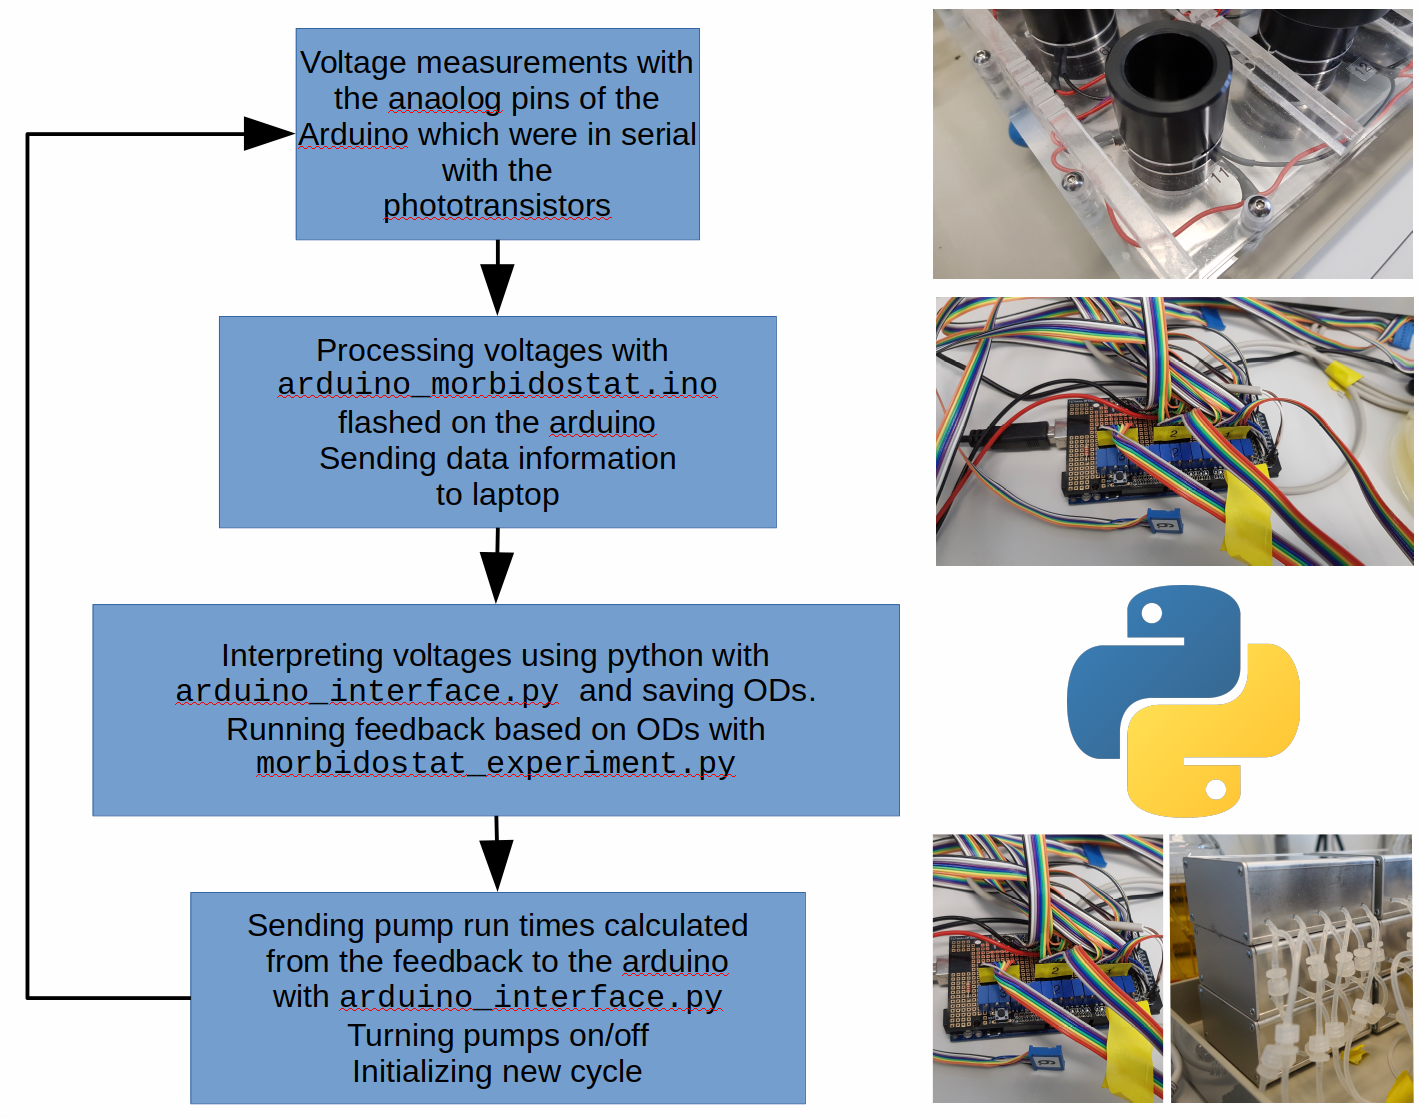
\includegraphics[scale=0.25]{flowchart.png}
	\caption{Overview of one cycle from the morbidostat.}
	\label{figure:flowchart}	
\end{figure}

\subsubsection{Feedback of the continuous mode} 
The feedback coded as a function in morbidostat\_experiment.py was very important since it was responsible for putting the culture under antibiotic pressure. The outcome of the feedback depended on the growth of the bacteria. Therefor the growth was calculated at the end of every cycle by calculating \textDelta OD according to the following formula:
\begin{center}
	$\Delta OD = (final\_OD[x_{cycles\_back}] - final\_OD[Cycle_{current})/x$
\end{center}
The final\_OD was calculated at the end of every cycle by averaging every OD measurment gathered over one cycle. As shown in the equation the difference between the final\_OD fromt the current cycle and the the final\_OD of x cycles back (x being typically 10) was calculated and divided by x.
As showin in Figure \ref{figure:feedback} the feedback did several comparisons before calculating an appropriate dose of drug. As a first step it checked if \textDelta OD was positive or negative. A negative \textDelta OD implied that the bacteria were dying. In order to prevent complete sterilization, media was getting added in this case. \\
When \textDelta OD was positive the bacteria were growing. Now it was important to not put the bacteria under selective pressure when the final\_OD of the cultures was very small (e.g. 0.03). If drug was added at this stage, this usually led to complete sterilization. That's why a threshold was introduced which was called drug\_dilution\_threshold. Therefor the next comparison as visible in Figure \ref{figure:feedback} was whether or not the final\_OD was higher or smaller than this threshold. If that was not the case the decision was to do nothing, which means that no fluid was added to the cultures. \\
However when the final\_OD was bigger than the threshold calculation of the appropriate dose was started.
This calculation depended on the MIC. Therefore the MIC had to be determined for the chosen bacteria and drug combination before the morbiostat experiment. Calculation of the concentration was divided into two equations consisting of an additive and a multiplicative component. The additive part was mainly important at the beginning of the experiment and was used to approximate a drug concentration in the vials similar to the MIC. Once the concentration in the vials was above the MIC the additive part was ignored. After that the current vial conentration was fed to an multiplicative equation. This equation multiplied the current drug concentration by the \textDelta OD which resulted in how much the drug concentration in the vial should be increased. This proved to be a good strategy, because fast growth meant stronger inhibition, but when the growth was very small and close to zero, the inhibition was not significantly increased. The multiplicative part also included other variables. For example a target\_OD was defined which was used to define which OD should not be exceeded. In general it was the goal to have the OD of the cultures close and steady to the target\_OD. \\
It was chosen to divide the outcome of the multiplicative component by this target\_OD. Therefor if the target\_OD was set to an high OD, inhibition was smaller than when set to a small OD. Furthermore variables had to be introduced to the multiplicative component which made it possible to make the feedback more aggressive or more sensitive.\\
Defining the target\_OD was a trade off of having a higher probability of mutations for a higher defined target\_OD, but keeping the culture at a high OD implemented fewer accuracy of the OD measurement caused by many dead cells.  


\begin{figure}
	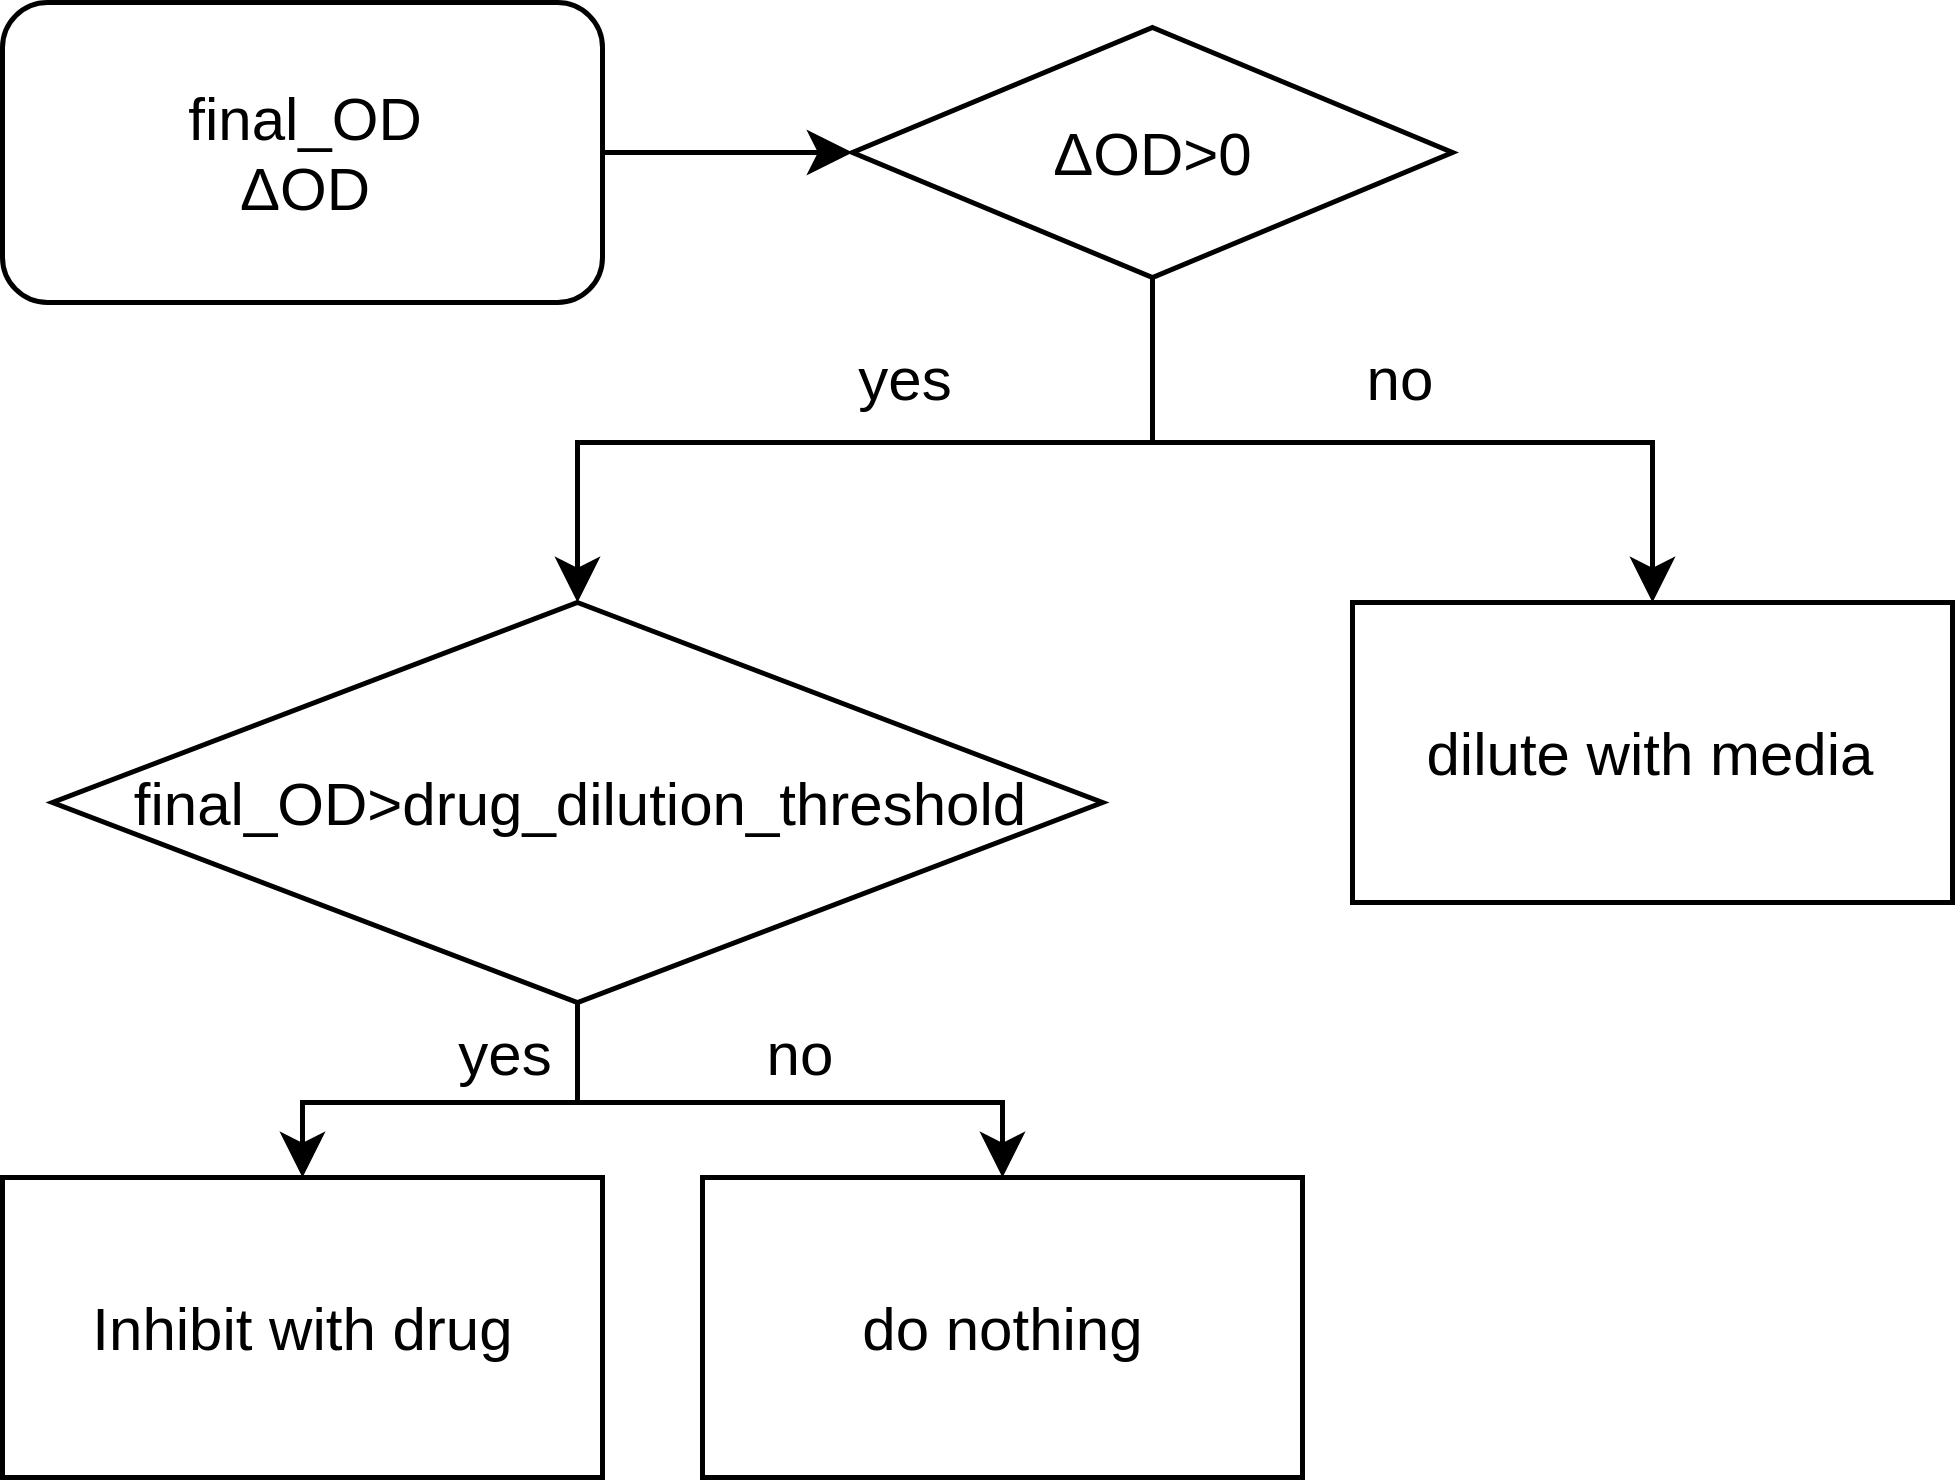
\includegraphics[scale=0.13]{feedback.png}
	\caption{Schematic overview of decisions involved in the feedback}
	\label{figure:feedback}
\end{figure}

\subsection{Hardware calibration}
\subsubsection{OD and pump calibration}
We chose 1/10 LB media and 9/10 $H_2O$ as a media for all experiments because the bacteria grew too fast when we used just LB media. All the culturing of the bacteria was done in a 37\degree C incubator. \\
For calibrating the OD measurements an overnight culure with K12 E. coli was inoculated in 5 ml diluted media. The next day the overnight culture was diluted 1/200 in 50 ml diluted media. After a few hours the OD of the culture was measured. Following OD standards were prepared with 18 ml diluted media in the vials for the morbidostat: 0.01 0.021 0.042 0.107 0.192 0.278\\
Then every vial with of a certain OD was placed in every vial holder. With the function calibrate\_OD from the morbidostat\_experiment.py script, a voltage measurement was done for every OD standard and every OD measuring unit. Because the voltage was measured for different ODs, the relation of voltage and OD could be described with a linear function. \\
For calibrating the pumps the function calibrate\_pumps from the morbidostat\_experiment.py was executed. This function demands the initial weight of every empty vial. After entering every weight, the function turned on every pump for 100 seconds. After that, the vials were weighted again and the values passed to the function which allowed precise calibration of each pump.
\label{section:OD_calibration}

\section{Safety aspects of morbidostat experiments}
Every experiment was done within the hypoxi-station. Next to temperature and $CO_2$ and nitrogen composition control, this ensured that in case of a leak no pathogens would get out in the open. \\
Based on the clinical strains from the University hospital of Basel and the sequencing data we produced several plasmids which we transformed into K-12. From two patients patient25 and patient33 we isolated the sequences coding for CTX-M-1 and OXA from the most susceptible sample. Next to the sequence coding for the ESBL we also took the upstream sequences up to the previous gene in order to ensure that we include the regulatory sequence. This resulted in three different plasmids. The patient number, ID of the plasmid and for which ESBL the sequence is coding is visible in Table \ref{table:plasmid}. All the plasmids were produced by gibson cloning. Every resulting clone was Illumina sequenced by the University hospital of Basel.

\begin{table}[H]
	\begin{tabular}{|c c c|}	
		\hline
		Patient & Plasmid ID & ESBL \\
		\hline
		25 & pEU22 & CTX-M-1 \\
		\hline
		25 & pEU23 & OXA \\
		\hline
		33 & pEU26 & OXA \\
		\hline
	\end{tabular}
	\label{table:plasmid}
	\caption{Produced plasmids}
\end{table}
\subsection{Gibson cloning}
\label{section:plasmid}
\subsubsection{Primer design}

\section{Experimental procedure for culturing with the continuous mode}
\subsection{MIC determination}
For experiments with the continuous mode the MIC of the antibiotic of interest had to be determined with the bacteria used for the experiment. That's because the feedback managing the inhibition is relied on the MIC. \\
Therefor 5 ml of MHB media was inoculated with the bacteria used for the actual experiment and cultured over night. The next day a 1/200 dilution in 20 ml MHB was prepared and cultured for a few hours. In the mean while a four fold concentration of the highest desired concentration was prepared. The growth of the diluted culture was constantly monitored by measuring the OD. When the OD of the diluted culture was at 0.08, a 1/100 dilution was done once again. From this final dilution 100 \textmu l was pipetted in every well from the 96 well expect in the wells from the last column of the plate. Additionally 100 \textmu l of MHB was added to every well. As a next step 100 \textmu l from the prepared drug solution was added to the first column of the plate. Then 100 \textmu l from this column were transferred to next column and mixed. This was repeated until the third last column. TThe second last column acted as a control of the cells, since no drug was added. The last column acted as a control for the media. After preparing the well plate it was incubated for 16 hours at 37 \degree \space on a shaker. To get an idea how many cells were used for the MIC determination $10^{-3}$ and $10^{-5}$ dilutions of the 1/100 diluted cell suspension were plated on LB plates.\\
After 16 hours the OD of every well was measured using a plate reader. The smallest concentration which inhibitted the growth was determined as the MIC. 
\label{section:mic_determination}


\subsubsection{Determination of growth rates}
For successfully culturing in the continuous mode appropriate dilution was helpful. A rather high dilution was helpful because an exchange of fluid prevented that too many bursted cell parts accumulated in the culture. Furthermore having a higher dilution helped to prevent the cultures from overgrowing. This was particularly useful at the beginning of the experiment because there was a lag until the antibiotic inhibited the growth. In order to determine an appropriate dilution it was necessary to record the growth rates of bacteria used for the experiment. Therefore all the growth rates were determined by culturing the bacteria used for the experiments in  the GROWTH\_RATE\_EXPERIMENT mode. The recorded growth rates were then fed to the \href{https://github.com/nahanoo/ESBL\_project/}{morbidostat\_simulator.py} script. This allowed to test different dilutions and to choose an appropriate cycle time. 
\label{section:growth_rates} 

\subsubsection{Sterilization of the morbidostat}
Before the experiment in the continuous mode could be started the morbidostat had to be sterilized. In order to do so all the tubing was flushed with 1 L of 3 \% citric acid, followd by 1 L of sterile water. After that 1 L of 3 \% bleach and 1 L of water was pumped through the tubing. All the media, drug bottles and vials including luer connections were autoclaved before the experiment.
\label{section:sterilization}


\subsection{Testing the feedback from the continuous culture mode}
An overnight culture was set up by inoculating 5 ml of diluted media with K12 XL1-Blue E. coli. The next day a 1/200 dilution in 200 ml was prepared and 18 ml of this suspension was pipetted in 18 sterile vials. \\
As described in \ref{section:growth_rates} the growth rates of K12 were determined over night and ideal dilution and cycle times tested with the simulator. A dilution factor of 0.94 and a cycle time of 12 minutes were chosen. 
As a drug we used amoxicillin, it's MIC was determined as 2 \textmu/ml according to the procedure in \ref{section:mic_determination}. As a starting concentration 6 \textmu/ml and 14 \textmu/ml were chosen for the drug bottles. Tubing, bottles and vials were sterilized according to the section \ref{section:sterilization}. 
From an other overnight culture of K12 XL1-Blue E. coli in 5 ml diluted media the morbidostat experiment was started in the continuous mode. Therefor the cells werle diluted to an OD of 0.015 in 18 ml. Every other day 200 \textmu of the suspension in the vials were transferred into new sterile vials filled with 18 ml diluted media. When a drug bottle was empty, the MIC was changed in the morbidostat\_experiment.py according to the concentration which was needed to strongly inhibit the growth. New drug concentrations were chosen based on the newly determined MIC. For the lower concentrated bottle a 3 fold MIC concentration, was chosen. For the higher concentrated drug bottle the concentration was set to 7 fold MIC. At day 4 of the experiment, samples were taken from every vial, by opening the vial in the hypoxi-station and transferring 200 \textmu into eppendorf tubes. Those samples were cultured over night in 5 ml diluted media and the next day the MIC was determined. The morbidostat experiment was stopped after 6 days.
\label{section:morb_test}

\subsection{Culturing K12 carrying ESBL plasmids with the morbidostat}
With the clones carrying ESBL plasmids (see Section \ref{section:plasmid}) we ran two continuous morbidostat experiments. Over night cultures of every clone were prepared in 3 ml LB with 3 \textmu L kanamycine. K12 was cultured over night in just 3 ml LB. The over night culture was diluted 200 fold the next day and the growth rates were determined (see Section \ref{section:growth_rates}). Additionally the MICs of every clone and K12 were determined as 2 \textmu g/ml (see Section \ref{section:mic_determination}). Based on the growth rates the dilution factor was set to 0.91 and the cycle time to 10 minutes. As drug concentrations 9 \textmu g/ml and 21 \textmu g/ml were chosen. MIC and drug concentrations were changed as described in Section \ref{section:morb_test}. The experiment was started with a starting OD of every culture of 0.015.
From every different clone a control was cultured where no antibiotic pressure was applied and the cultures were diluted with media to a fixed OD. This fixed OD (target\_OD) was set to 0.12. Different modes were chosen for following vials.

\begin{table}[H]
	\begin{tabular}{|c c c|}	
		\hline
		Vial & Plasmid & Mode \\
		\hline
		1 & pEU26\_OXA & continuous \\
		\hline
		2 & pEU26\_OXA & continuous \\
		\hline
		3 & pEU23\_OXA & continuous \\
		\hline
		4 & pEU23\_OXA & continuous \\
		\hline
		5 & pEU23\_OXA & continuous \\
		\hline
		8 & pEU26\_OXA & continuous \\
		\hline
		9 & pEU23\_OXA & fixed OD \\
		\hline
	\end{tabular}
	\quad
		\begin{tabular}{|c c c|}	
		\hline
		Vial & Plasmid & Mode \\
		\hline
		1 & pEU26\_OXA & continuous \\
		\hline
		2 & pEU23\_OXA & continuous \\
		\hline
		3 & pEU22\_CTX-M-1 & continuous \\
		\hline
		4 & pEU22\_CTX-M-1 & continuous \\
		\hline
		5 & pEU22\_CTX-M-1 & continuous \\
		\hline
		7 & K12 & continuous \\
		\hline
		8 & pEU22\_CTX-M-1 & fixed OD \\
		\hline
		9 & pEU26\_OXA & fixed OD \\
		\hline
		10 & pEU26\_OXA & fixed OD \\
		\hline
	\end{tabular}
	\caption{Left table: Experiment 01, right table: Experiment 02}
\end{table}

Experiment 01 ran for two days and only samples were taken from the last day. Experiment 02 ran for six days and samples were collected every day. For sampling 1 ml of every vial was transferred into an eppendorf tube within the hypoxi-station. The samples was centrifuged for 10 minutes at 13000 rpm and the resulting cell pellet resuspended in 200 \textmu LB media containing 20 \% glycerol. The resuspended cells were frozen and kept as stocks. \\
From the 01 experiment the stocks of every vial from the last sample day were handed over to the Unversity hospital of Basel for Illumina sequencing. From the 02 experiments samples from the second sample day of vial 3,4,5,7 and 8 were chosen for sequencing. Additionally every sample from the last sampling day of the 02 experiments were handed over for Illumina sequencing. 